% !TEX encoding = UTF-8 Unicode
%!TEX root = thesis.tex
% !TEX spellcheck = en-US
%%=========================================
\chapter{Introduction}
Semantic segmentation and feature extraction in remote sensing has been a field of research for many decades. The ability to extract geospatial information directly from satellite imagery has been crucial for areas such as environmental and demographic research. Furthermore, a vast development within the field of machine learning and artificial intelligence the last years has enabled many researchers to find useful applications of such algorithms within their scientific fields.

With new satellite technology providing frequently updated imagery, with resolutions less than 0.5 meters, the amount of data that can be extracted is almost incomprehensible. This paper focuses on how automatic height estimation of ground objects can be achieved through remote sensing, semantic image segmentation, and different height estimation techniques.

The primary goal of this study is to investigate different methods for automatic detection and height retrieval of the roofs of oil tanks in Cushing, Oklahoma. By knowing the height difference between the tanks floating roofs and their actual height, it is possible to calculate their inventory.

%%=========================================
\section{Background}
% In this section, you should present the problem that you are going to investigate or analyze; why this problem is of interest; what has, so far, been done to solve the problem, and which parts of the problem that remain.

Satellites have been collecting earth observation data for decades. Since the satellite Explorer 6 took the first picture of the earth in 1959, millions of satellite images have been captured, processed and stored \cite{Esa2009a}. This information has been difficult to access, and even harder to analyze when accessible. However, during the last decade, the development of machine learning based methods for Earth Science applications has experienced a considerable leap forward \cite{Lary2010}.

In 2014 the first satellite in the new family of earth observation satellites, called the Sentinels, was launched from Kourou, French Guiana. Since then seven different constellations, each consisting of two satellites,  have been launched, and are now orbiting and monitoring the earth's surface. The goal of these satellites is to produce a continuous stream of timely data for Europe's Copernicus program, which will be used for environmental monitoring. The different constellations have different missions when it comes to providing datasets for the Copernicus Service. While some are focused on specific data, such as monitoring the earth's atmosphere, other constellations offer more general data, such as multi-spectral, high-resolution imagery of the earth's surface. In order to maximize the usage of these temporal datasets, they have all been provided free of charge to the public. Other satellite constellations such as SkySat \citep{Planet2017} and WorldView \citep{DigitalGlobe2017} provide even more accurate satellite imagery, with submeter resolutions. With these satellites providing frequently updated imagery over most parts of the earth's surface, the amount of earth observation data that can be observed is enormous. 

The development of these satellite constellations means that data that earlier required manual measurements to be analyzed, now can be gathered, processes and analyzed automatically at a high phase. One field where this can provide valuable information is within the oil industry.

Cushing Oklahoma is the major trading hub and famous price settlement point for West Texas Intermediate of the New York Mercantile Exchange. With inventory numbers not being continuously updated by Energy Information Administration (EIA), there exists a potential in retrieving these numbers automatically through remote sensing.

\begin{figure}[!h]
	\centering
	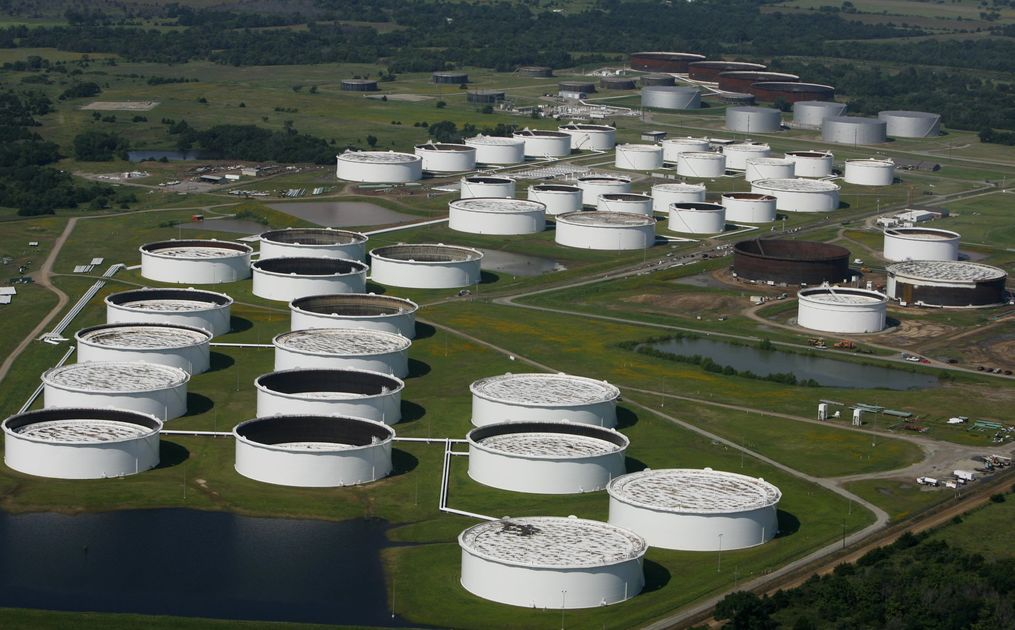
\includegraphics{fig/cushing_oklahoma.jpg}
	\caption{Oil tanks with different amounts of oil inventory}
	\label{fig:cushingoklahoma}
\end{figure}

%%=========================================
\section{Problem}
%You should define your problem in a clear an unambiguous way and explain why this is a problem, why it is of interest---and to whom. It is also important to delimit the problem area.

The paper aims to answer if it is possible, with today's methods and satellite technology to automatically provide frequently updated estimations of the total inventory of all the crude oil tanks in Cushing, Oklahoma.

%%=========================================
\section{Approach}
%Here you should describe the (scientific) approach and experiments that you will use or have used to solve the problem and meet your objectives and tasks. Experiments may in this context relate analyses you need to carry out in order to investigate a specific hypothesis, task objective, or similar. You should specify the approach and experiments for each objective and/or task. It is preferred that you supplement your explanation of the approach with an illustration.

This paper will focus on investigating the theory and previous work related to semantic segmentation of satellite images and techniques for height detection using data collected through remote sensing. By combining these two fields of research, it is theorized that it can be possible to automatically locate and estimate the inventory of oil tanks in Cushing, Oklahoma.

\subsection*{Semantic segmentation}
Regarding semantic segmentation, the paper discusses different approaches ranging from standard methods, such as the Hough transform to newer, more advanced techniques such as image segmentation using convolutional neural networks. The goal is to present the strengths and weaknesses of the different methods, to determine which one is most suitable for the task at hand.

\subsection*{Height estimation}
There are also a large variety of different methods for height estimation using data from satellite imagery. While the methods investigated related to semantic segmentation only focus on multispectral images, both techniques using radar images and multispectral imaged are considered for height estimation. The methods that are examined are SAR, InSAR and shadow measurements.

%%=========================================
\section{Limitations}
%In this section you describe the limitations of your study. These may be related to the study object (physical limitations, operational limitations), to the environmental and operational conditions, to the thoroughness of the analysis, and so on.

This study is conducted as a literature review and does not present any implementation of the methods that are investigated.

%%=========================================
\section{Outline}
%Here, you give an overview of how the remaining part of the report is organized. A proposed structure of the main chapters in the report can be as follows (note that some chapters are not numbered):
The remaining part of this paper consists of the following chapters:

\begin{itemize}
\item Chapter 2. Theoretical background: This chapter gives a theoretical background of the different methods that are investigated later in the paper. It provides the necessary knowledge required to understand the various methods presented in related work.
\item Chapter 3. Related Work: In this chapter, the previous work relevant to this paper is presented. It includes standard methods for image segmentation, an overview of the advances in convolutional neural networks and how they can be used for image segmentation. Furthermore, different works related to height estimation of buildings are presented.
\item Chapter 4. Evaluating the methods: The focus of this chapter is to evaluate and compare the different methods that have been investigated in the previous chapters.
\item Chapter 5. Conclusions, discussion, and ideas for further work: A conclusion is presented based on the previous chapters and some future work is presented.
\item Bibliography
\end{itemize}